% !Mode:: "TeX:UTF-8"
% !TEX root = ..\thesis.tex
\chapter{研究对象基本情况}
本文以某汽车电子有限公司的装配车间为研究对象,进行调研。本章将介绍该公司车间的基本情况,并对现有装配线调度情况进行初步分析。
\section{公司基本情况}
该汽车电子有限公司主要产品为车用电子电器开关、控制模块、控制面板等,是美国通用、德国大众、一汽大众、上海大众、上海通用、上海汽车、长安福特、北京现代、一汽轿车、奇瑞汽车、哈飞集团等国内外40余家汽车主机厂的专业定点配套供应商,配套的代表性车型有奥迪A6(L)、奥迪A4(L)、奥迪Q5、迈腾、君越、宝来、帕萨特、奔腾、红旗、马自达M6、景程、荣威、明锐、凯越、捷达、桑塔纳等系列轿车,以及卡车、轻型车、微型车等,产品型号达6000余种。

\section{装配车间作业}
该公司装配车间有多条作业流水线,每条流水线负责某一种品牌单项产品的总装流程,生产较为固定,产线间的工装设备及流程相似但不相同,不同客户的订单基本不在相同的产线上装配。

装配作业采用同步装配流水线方式,将装配过程分为多个作业单元,并安排在流水线的相应工位上,车体在移动中装配,各工位同时作业。不同产线间会出现相同的作业内容,但考虑到装配过程的连续性,需要重复安排人员及设备。

该公司采用面向订单生产,订单从接受到交付的流程如\reff{fig:orderflow}所示,其中虚线框内为装配车间的作业,客户源较为稳定,其需求特点使得装配作业呈现为多品种小批量的生产方式。在没有订单或者订单较少时,为了不让生产线停下来,需要进行工厂内部的计划生产,而订单较多时需要加班作业。
\begin{figure}[h]
\centering
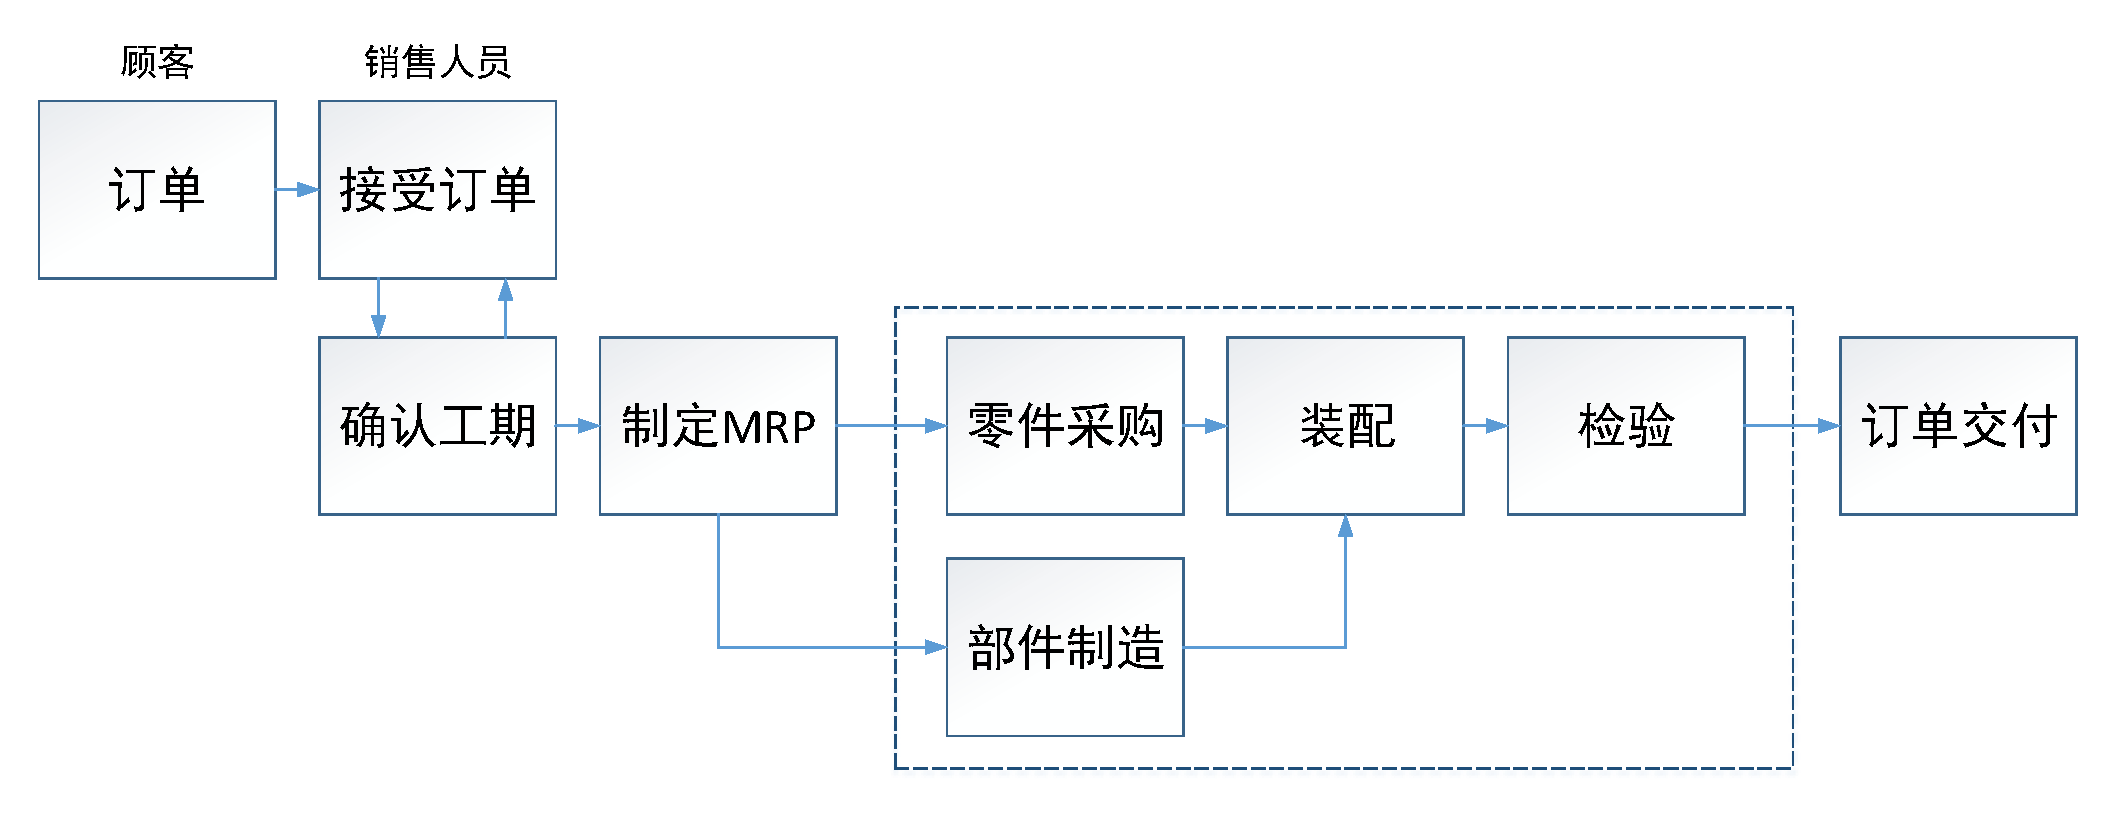
\includegraphics[width = 12cm]{orderflow.pdf}
\caption{现行作业信息流\label{fig:orderflow}}
\end{figure}

\section{产线调度现状}
当前该公司装配车间采用专线生产的方式,即客户的订单在其专用的流水线上进行生产作业,当同一客户有多个订单下达时,按照先到先服务(FCFS)的规则进行调度安排,多条产线并行作业互不干扰。

订单或任务到达时,如果有产线空闲可用,则立马对其根据进行生产准备,然后开始装配生产。若所有产线都在处理订单,那么将该订单安排入具有最早的最迟队列任务交货期的队列(队列生成逻辑如\reff{fig:queuelog}所示),然后按照预定的调度规则(FCFS)进行生产处理,现行调度的产线如\reff{fig:3nowschedule}所示。

\begin{figure}[h]
\floatsetup{floatrowsep = fill}
\begin{floatrow}[2]
\ffigbox[\FBwidth]{\caption{队列生成逻辑\label{fig:queuelog}}}{\includegraphics[width = 7cm,trim = 0 20 0 0]{queuelogic.pdf}}
\ffigbox[\Xhsize]{\caption{3条生产线的现行调度\label{fig:3nowschedule}}}{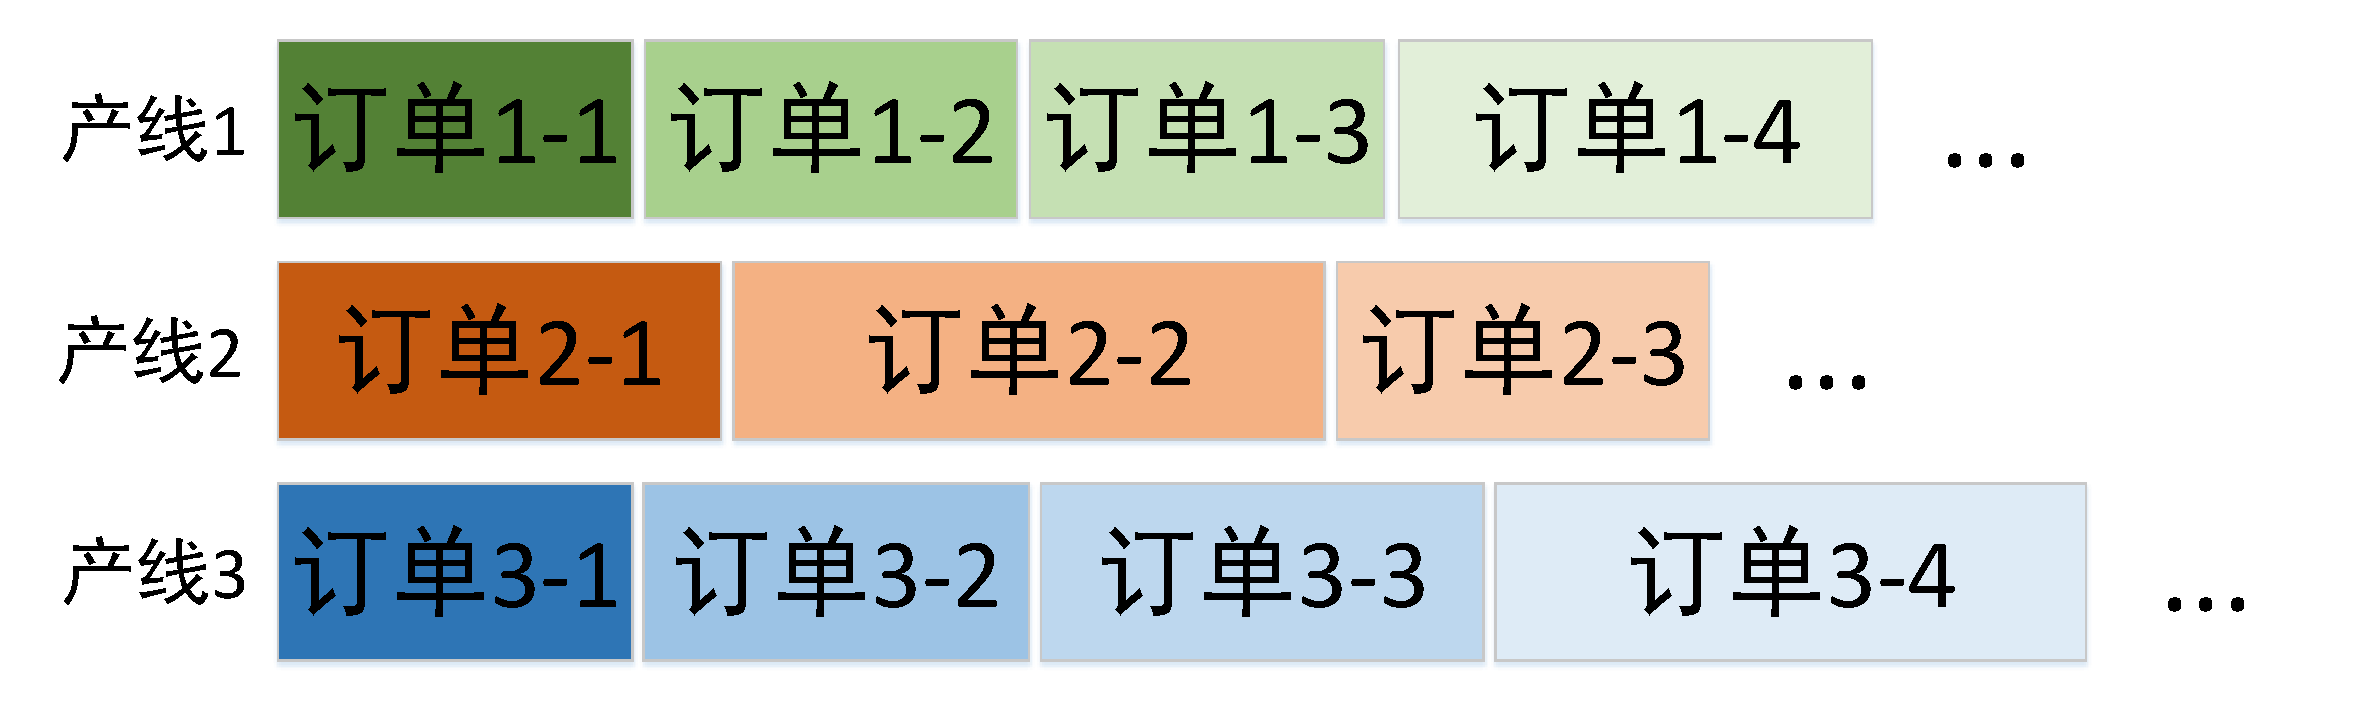
\includegraphics[width = 9cm,trim = 0 -180 0 0]{orderschedulenow.pdf}}
\end{floatrow}
\end{figure}
\section{小结}
本章...
产线调度现状反映了一些问题,例如 ,在下一章将具体描述和分析这些问题。产线调度现状反映了一些问题,例如 ,在下一章将具体描述和分析这些问题。产线调度现状反映了一些问题,例如 ,在下一章将具体描述和分析这些问题。产线调度现状反映了一些问题,例如 ,在下一章将具体描述和分析这些问题。产线调度现状反映了一些问题,例如 ,在下一章将具体描述和分析这些问题。产线调度现状反映了一些问题,例如 ,在下一章将具体描述和分析这些问题。产线调度现状反映了一些问题,例如 ,在下一章将具体描述和分析这些问题。产线调度现状反映了一些问题,例如 ,在下一章将具体描述和分析这些问题。产线调度现状反映了一些问题,例如 ,在下一章将具体描述和分析这些问题。产线调度现状反映了一些问题,例如 ,在下一章将具体描述和分析这些问题。产线调度现状反映了一些问题,例如 ,在下一章将具体描述和分析这些问题。产线调度现状反映了一些问题,例如 ,在下一章将具体描述和分析这些问题。产线调度现状反映了一些问题,例如 ,在下一章将具体描述和分析这些问题。产线调度现状反映了一些问题,例如 ,在下一章将具体描述和分析这些问题。产线调度现状反映了一些问题,例如 ,在下一章将具体描述和分析这些问题。产线调度现状反映了一些问题,例如 ,在下一章将具体描述和分析这些问题。产线调度现状反映了一些问题,例如 ,在下一章将具体描述和分析这些问题。